\chapter{Eigenwerte und Eigenvektoren\label{chapter-eigen}}
\index{Eigenwert}
\index{Eigenvektor}
\rhead{Eigenwerte und Eigenvektoren}
In vielen Anwendungen hat man ein Gleichungssystem der Form
$$Ax=\lambda x$$
zu l"osen, wobei nicht nur der Spaltenvektor $x$, sondern auch der
Parameter $\lambda$ unbekannt sind. Nat"urlich kann man ein solches
Problem immer umschreiben in die Form
$$(A-\lambda E) x=0,$$
also ein Gleichungssystem, welches entweder gar keine, oder dann
unendlich viele L"osungen hat. Daher interessiert die Frage 
ganz besonders, f"ur welche $\lambda$ eine nicht triviale L"osung m"oglich ist.

In diesem Kapitel geht es darum, diese sogenannten Eigenwerte $\lambda$
und die zugeh"origen L"osungsvektoren, die Eigenvektoren, zu finden. Dieses
Problem ist von grosser praktischer Bedeutung, sehr viele Anwendungsproblem
lassen sich darauf zur"uckf"uhren. Es lohnt sich also, dieses Problem
effizient l"osen zu k"onnen. Beispiele:
\begin{compactitem}
\item L"osung von linearen Differenzengleichungen
\index{lineare Differenzengleichung}
\item L"osung von linearen Differentialgleichungen beliebiger Ordnung
\index{lineare Differentialgleichung}
\item Schwingungen eines Bauwerks oder einer Maschine: die Bewegung wird durch
eine partielle Differentialgleichung beschrieben, die Schwingungsfrequenzen
werden durch die Eigenwerte gegeben. Um Resonanzen und damit die Zerst"orung
zu verhindern, muss der Ingenieur die Eigenfrequenzen
berechnen k"onnen.
\index{Schwingung}
\index{Eigenfrequenz}
\item Resonanzen eines Hohlraumresonators: die Felder im Hohlraumresonator
werden durch eine partielle Differentialgleichung beschrieben.
Die Eigenfrequenzen sind Eigenwerte, der Ingenieur kann durch Ver"anderung
der Geometrie des Hohlraumes das Frequenzsprektrum anpassen.
\index{Resonanz}
\index{Hohlraumresonator}
\index{partielle Differentialgleichung}
\index{Frequenzspektrum}
\item
\index{Akustik}
In der
Akustik strebt man eine m"oglichst gleichm"assige Verteilung der Eigenfrequenzen
eines Konzertsaals an, um dem Zuh"orer ein m"oglichst ausgewogenes Klangbild
zu bieten.
\item Klangspektrum eines Musikinstruments: Die Schwingungen eines Musikinstruments
werden durch eine partielle Differentialgleichung beschrieben, die
Eigenwerte beschreiben die Oberton-Frequenzen, die im Klangspektrum des
Instruments vertreten sind.
\index{Klangspektrum}
\end{compactitem}
Bis auf das erste Beispiel stehen Ihnen die mathematischen Mittel noch nicht
zur Verf"ugung, auch nur die Problemstellung zu formulieren, daher beginnen
wir mit einer Differenzengleichung als einf"uhrendes Beispiel.

\section{Problemstellung}
In diesem Kapitel gehen wir immer von einer $n\times n$-Matrix $A$ aus.

\medskip
{\parindent0pt \bf Problem:} Finde Vektoren $x\in\mathbb R^n$ und
Zahlen $\lambda\in\mathbb R$ so, dass $Ax=\lambda x$.
\medskip

{\parindent0pt Diese Problemstellung ist nicht ganz klar:}
\begin{compactitem}
\item Der Vektor $x=0$ ist immer eine L"osung, das Problem ist also
nur dann interessant, wenn Vektoren $x\ne 0$ verlangt werden.
\item Der Vektor $x$ ist nicht eindeutig bestimmt. Gilt $Ax=\lambda x$,
dann gilt dasselbe auch f"ur $y=\mu x$:
\[
Ay= A(\mu x)=\mu Ax=\mu\lambda x = \lambda (\mu x)=\lambda y.
\]
Der Vektor $x$ kann also bestenfalls bis auf eine Vielfaches
bestimmt werden.
\end{compactitem}

\index{Eigenwert}
\index{Eigenvektor}
\begin{definition}
Ein Vektor $v \in \mathbb R^n$ heisst Eigenvektor der $n\times n$-Matrix $A$
zum Eigenwert $\lambda$, wenn $v\ne 0$ und $Av=\lambda v$ gilt.
\end{definition}

\begin{beispiel}
Die Matrix
$$\begin{pmatrix}
3&0&0\\
0&5&0\\
0&0&7
\end{pmatrix}$$
hat die Eigenwerte $3$, $5$ und $7$, mit den Eigenvektoren
\[
\begin{pmatrix}
1\\0\\0
\end{pmatrix}
,
\begin{pmatrix}
0\\1\\0
\end{pmatrix}
,
\begin{pmatrix}
0\\0\\1
\end{pmatrix}
\]
\end{beispiel}

\begin{hilfssatz}
\index{Diagonalmatrix}
Die Diagonalmatrix
$$
\operatorname{diag}(\lambda_1,\dots,\lambda_n)
=\begin{pmatrix}
\lambda_1&\dots&0\\
\vdots&\ddots&\vdots\\
0&\dots&\lambda_n
\end{pmatrix}
$$
hat die Eigenwerte $\lambda_1,\dots,\lambda_n$, die Einheitsvektoren
$e_i$ sind Eigenvektoren zum Eigenwert $\lambda_i$.
\end{hilfssatz}
Offenbar ist dies ein besonders einfacher Fall, die Basisvektoren sind
alle Eigenvektoren. Es gibt einige Klassen von Matrizen, bei denen es
immer m"oglich ist, eine Basis aus Eigenvektoren zu w"ahlen. Hat die
$n\times n$-Matrix $A$ $n$ linear unabh"angig Eigenvektoren $v_1,\dots,v_n$
mit Eigenwerten $\lambda_1,\dots,\lambda_n$, dann kann man die Wirkung
der Matrix $A$ auf einen beliebigen Vektor $x=\alpha_1v_1+\dots+\alpha_nv_n$
sofort berechnen:
$$Ax=\alpha_1Av_1+\dots+\alpha_nAv_n=\alpha_1\lambda_1v_1+\dots+\alpha_n\lambda_nv_n.$$
In der Basis $\{v_1,\dots,v_n\}$ hat $A$ also die Matrix
$$
A=\operatorname{diag}(\lambda_1,\dots,\lambda_n)
=
\begin{pmatrix}
\lambda_1&\dots&0\\
\vdots&\ddots&\vdots\\
0&\dots&\lambda_n
\end{pmatrix}.
$$
\begin{definition}
\index{diagonalisierbar}
\index{diagonalisieren}
Eine Matrix $A$ heisst diagonalisierbar, wenn es eine Basis aus
Eigenvektoren gibt.
\end{definition}

Wir haben also die Gleichung $Ax=\lambda x$ zu l"osen. W"are 
$\lambda$ bekannt, k"onnten wir das Problem in ein Standardproblem
umwandeln:
\[
Ax=\lambda x\qquad\Rightarrow\qquad Ax-\lambda Ex=(A-\lambda E)x=0
\]
gesucht ist also ein nicht verschwindende L"osung des homogenen
Gleichungssystems mit
Matrix $A-\lambda E$. Nur kennen wir $\lambda$ nicht. Allerdings
liefert gerade die Bedingung, dass wir ein nicht verschwindende
L"osung des homogenen Systems finden wollen ein Kriterium zur
Bestimmung von $\lambda$: $A-\lambda E$ muss singul"ar sein.
Das Eigenwertproblem wird also in zwei Schritten gel"ost:
\begin{compactenum}
\item Bestimmung der m"oglichen Eigenwerte: f"ur welche Werte von $\lambda$
ist $A-\lambda E$ singul"ar?
\item Bestimmung der Eigenvektoren zu gegebenem Eigenwert: Finde die
L"osungen von $(A-\lambda E)x=0$. Hierzu kann der Gauss-Algorithmus
verwendet werden, oder in einfachen F"allen auch die Cramersche Regel.
\end{compactenum}
Die folgenden Einf"uhrungsbeispiele sollen zeigen, wie das Eigenwertproblem
in der Praxis auftaucht und gel"ost werden kann. 

\section{Zwei Einf"uhrungsbeispiele}
\subsection{Federkette}
\begin{figure}
\begin{center}
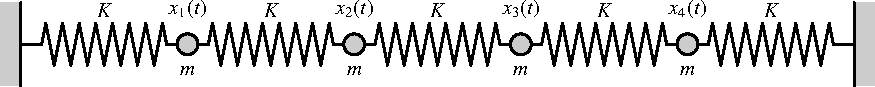
\includegraphics[width=\hsize]{images/e-1}
\end{center}
\caption{Federkette}
\index{Federkette}
\end{figure}
Wir betrachten $n$ gleiche Massen $m$, welche in einer Kette mit gleich
starkten Federn miteinenader verbunden sind. Am Ende sind die Massen
ebenfalls mit einer Feder verankert.
Die Massen sollen sich nur entlang der Achse der Federkette bewegen k"onnen.
Die Variablen $x_i(t)$ sind Funktionen, die die Auslenkung der Masse mit
Nummer $i$ zur Zeit $t$ aus der Ruhelage beschreibt. Die Bewegungsgleichung sagt,
dass die zweite Ableitung der Position die von den Federn bewirkte Kraft
ist. Die Federkraft ist proportional zum Auslenkungsunterschied
$x_{i+1}(t)-x_i(t)$ f"ur die ``rechte'' Feder, bzw.~
$x_{i}(t)-x_{i-1}(t)$ f"ur die ``linke'' Feder.
Die Kraft ist also
\begin{align*}
m\frac{d^2x_i(t)}{dt^2}
&=K((x_{i+1}(t)-x_i(t))-(x_i(t)-x_{i-1}(t)))\\
&=K(x_{i+1}(t)-2x_i(t)+x_{i-1}(t))
\end{align*}
Aus der Erfahrung wissen wir, dass so eine Federkette schwingt, wir nehmen also
an, dass wir eine L"osung in der Form $x_i(t)=x_i(0)\sin\omega t$ finden
k"onnen. Setzen wir dies ein, erhalten wir die Gleichungen
$$
-m\omega^2\sin\omega t x_i(0)=K(x_{i+1}(0)-2x_i(0)+x_{i-1}(0))\sin\omega t.
$$
Da diese Gleichung muss f"ur alle Zeitpunkte gelten muss, gilt sie auch f"ur
Zeitpunkte, an denen $\sin\omega t\ne 0$, so dass man durch $\sin\omega t$
teilen kann:
$$
-m\omega^2 x_i(0)=K(x_{i+1}(0)-2x_i(0)+x_{i-1}(0)).
$$
F"ur die Endpunkte der Kette gelten einfachere Formeln. Auf die Masse $1$
wirkt die Feder links mit der Kraft $-Kx_1(t)$, die Feder rechts "ubt die
Kraft $K(x_2(t)-x_1(t))$ aus, so dass die Bewegungsgleichung hier zu
$$
-m\ddot x_1(t)=K(-2x_1(t)+x_2(t)),
$$
die Gleichung f"ur die Anfangswerte wird
$$
\omega^2 x_1(0)=-\frac{K}{m}(-2x_1(0)+x_2(0)),
$$
und analog am anderen Ende des Intervals.

Diese Gleichung soll jetzt auch noch in Matrizenform geschrieben werden.
Die Anfangswerte $x_i(0)$ fassen wir in einen Vektor $x(0)$ zusammen.
Die rechte Seite der Gleichung wird durch die Wirkung der $n\times n$-Matrix
$$
\Delta=
-\frac{K}{m}
\begin{pmatrix}
-2&1&0&0&0&\dots&&&0\\
1&-2&1&0&0&&&&\\
0&1&-2&1&0&&&&\\
0&0&1&-2&1&&&&\\
\vdots&&&&&\ddots&&\\
 &&&&&&-2&1&0\\
 &&&&&&1&-2&1\\
0&&&&&&0&1&-2
\end{pmatrix}
$$
beschrieben.

Unbekannt ist jetzt offenbar, welche Werte $\omega$ "uberhaupt eine nicht-%
triviale L"osung erm"oglichen, also einen Vektor $x$ mit der Eigenschaft
$$
\Delta x=\lambda x
$$
mit $\lambda=\omega^2$. Wenn wir die zul"assigen $\lambda$ bestimmen k"onnen,
f"ur die sich eine L"osung $x$ finden l"asst, dann kennen wir offenbar auch
die Eigenfrequenzen, mit denen die Federkette schwingen kann.

\subsubsection{Zwei Massen}
F"ur nur zwei Massen wird die Matrix $\Delta$ zu
\[
\Delta=\begin{pmatrix}
2&-1\\
-1&2
\end{pmatrix}.
\]
Um die Werte $\lambda$ zu finden, f"ur die $\Delta-\lambda E$ singul"ar
wird, k"onnen wir das Determinanten-Kriterium verwenden:
\begin{align*}
\left|\;\begin{matrix}
2-\lambda&-1\\-1&2-\lambda
\end{matrix}\;\right|
&=(2-\lambda)^2-1=\lambda^2 -4\lambda+3=0.
\\
\Rightarrow\qquad
\lambda_{\pm}&=2\pm\sqrt{2^2-3}=\begin{cases}3\\1\end{cases}
\end{align*}
Die Eigenvektoren sind L"osungen des homogenen Gleichungssystems mit
Koeffizientenmatrix $\Delta-\lambda E$. 
Einen Vektor im Nullraum
von
\begin{align*}
\lambda&=\lambda_-=1:&
(\Delta -1\cdot E)v_-&=
\begin{pmatrix}
1&-1\\-1&1
\end{pmatrix}v_-=0
&
v_-&=\begin{pmatrix}1\\1\end{pmatrix}
\\
\lambda&=\lambda_+=3:&
(\Delta -3\cdot E)v_+&=
\begin{pmatrix}
-1&-1\\-1&-1
\end{pmatrix}v_+=0
&
v_+&=\begin{pmatrix}1\\-1\end{pmatrix}
\end{align*}
\begin{figure}
\begin{center}
\begin{tabular}{ll}
$\lambda=\lambda_-:$&%
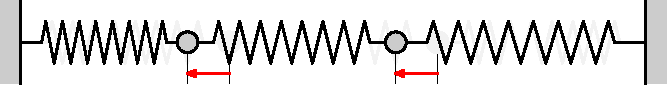
\includegraphics{images/e-4}\\%
&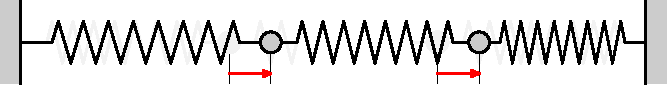
\includegraphics{images/e-5}\\%
\\
$\lambda=\lambda_+:$&%
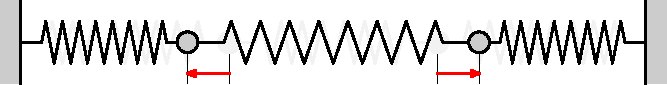
\includegraphics{images/e-2}\\%
&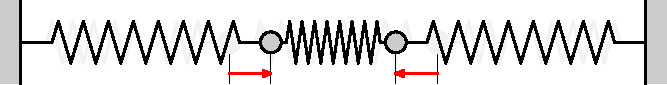
\includegraphics{images/e-3}%
\end{tabular}
\end{center}
\caption{Schwingungsmodi einer Federkette mit zwei Massen ( $n=2$)\label{n2modi}}
\end{figure}%
Es gibt also zwei Schwingungsmodi, in
Abbildung~\ref{n2modi} werden jeweils die beiden Extremlagen 
gezeigt.
Bei der langsamen Schwingung mit Kreisfrequenz
$\omega_-=\sqrt{\lambda_-}=1$ bewegen sich die Massen gleichphasig,
was auch angezeigt wird durch die gleichen Vorzeichen
der Komponenten von $v_-$.
Bei der schnellen Schwingung mit Kreisfrequenz
$\omega_+=\sqrt{\lambda_+}=\sqrt{3}\simeq 1.732$ bewegen sich die 
beiden Massen gegenphasig, ausgedr"uckt auch durch
die verschiedenen Vorzeichen der Komponenten von $v_+$.

\subsubsection{Drei Massen}
Auch f"ur drei Massen l"asst sich das Eigenwertproblem noch
``von Hand'' l"osen. Wir verwenden wieder das Determinanten-Kriterium
\begin{align*}
\det(\Delta -\lambda E)&=\left|\;
\begin{matrix}
2-\lambda&-1&0\\
-1&2-\lambda&-1\\
0&-1&2-\lambda
\end{matrix}
\;\right|
=-\lambda^3+6\lambda^2-10\lambda+4=-(\lambda-2)(\lambda^2-4\lambda+2)
\\
\Rightarrow\qquad
\lambda_1&=2\\
\lambda_{2,3}&=2\pm\sqrt{2^2-2}=2\pm\sqrt{2}
\end{align*}
F"ur die Eigenvektoren finden wir
\begin{align*}
\lambda&=\lambda_1=2:
&
(\Delta - 2\cdot E)v_1&=\begin{pmatrix}
0&-1&0\\
-1&0&-1\\
0&-1&0\end{pmatrix}v_1
=0&v_1&=\begin{pmatrix}1\\0\\-1\end{pmatrix}
\\
\lambda&=\lambda_2=2+\sqrt{2}:
&
(\Delta -(2+\sqrt{2})E)v_2&=\begin{pmatrix}
-\sqrt{2}&-1&0\\
-1&-\sqrt{2}&-1\\
0&-1&-\sqrt{2}
\end{pmatrix}v_2=0&
v_2&=\begin{pmatrix}
1\\-\sqrt{2}\\1
\end{pmatrix}
\\
\lambda&=\lambda_3=2-\sqrt{2}:
&
(\Delta -(2-\sqrt{2})E)v_2&=\begin{pmatrix}
\sqrt{2}&-1&0\\
-1&\sqrt{2}&-1\\
0&-1&\sqrt{2}
\end{pmatrix}v_2=0&
v_2&=\begin{pmatrix}
1\\\sqrt{2}\\1
\end{pmatrix}
\\
\end{align*}
\begin{figure}
\begin{center}
\begin{tabular}{l}
geringste Eigenfrequenz: $\lambda=\lambda_3$:\\
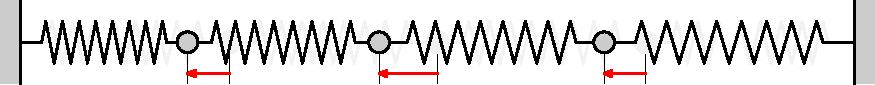
\includegraphics[width=\hsize]{images/e-8}\\
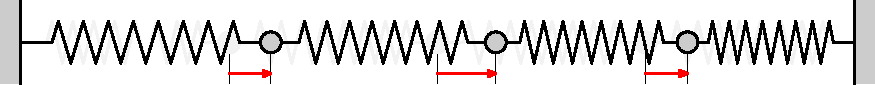
\includegraphics[width=\hsize]{images/e-9}\\
\\
mittlere Eigenfrequenz: $\lambda=\lambda_1$:\\
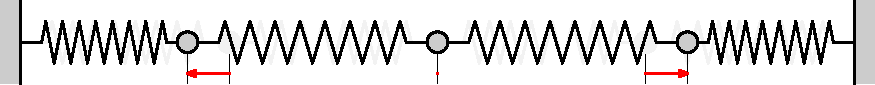
\includegraphics[width=\hsize]{images/e-6}\\
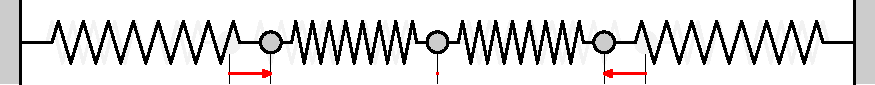
\includegraphics[width=\hsize]{images/e-7}\\
\\
h"ochste Eigenfrequenz: $\lambda=\lambda_2$:\\
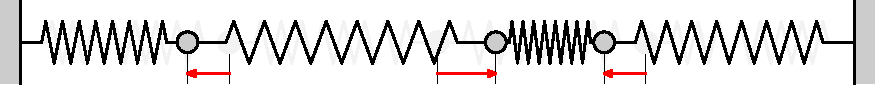
\includegraphics[width=\hsize]{images/e-10}\\
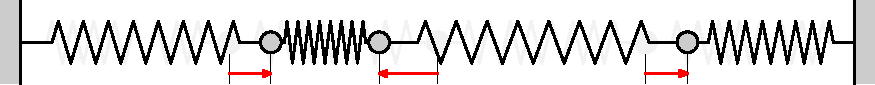
\includegraphics[width=\hsize]{images/e-11}
\end{tabular}
\end{center}
\caption{Schwingungsmodi einer Kette mit drei Massen ($n=3$)\label{n3modi}}
\end{figure}%
Diesmal gibt es drei Schwingungsmodi, von denen in Abbildung~\ref{n3modi}
wieder jeweils die Extremlagen dargestellt sind. Zur geringsten Frequenz
$\omega_3=\sqrt{\lambda_3}=\sqrt{2-\sqrt{2}}\simeq 0.7654$
geh"ort eine Schwingung, bei der alle drei Massen in Phase
hin- und herschwingen, wobei die mittlere Masse eine 41\% 
gr"ossere Amplitude hat (Abbildung~\ref{n3modi} unten).
Zur h"ochsten Frequenz
$\omega_2=\sqrt{\lambda_2}=\sqrt{2+\sqrt{2}}\simeq 1.848$
geh"ort eine Schwingung, bei der die "ausseren Massen in Phase sind,
aber gegenphasig zur mittleren Massen schwingen, die wieder etwa
41\% gr"ossere Amplitude hat (Abbildung~\ref{n3modi} mitte).
Die mittlere Frequenz $\omega_1=\sqrt{\lambda_1}=\sqrt{2}\simeq 1.414$
geh"ort zu einer Schwingung, bei der die mittlere Masse stehenbleibt,
w"ahrend die "ausseren beiden Massen gegenphasig schwingen (Abbildung~\ref{n3modi} oben).

\subsubsection{Numerische Resultate}
Mindestens numerisch kann man jetzt bereits viele bekannte
Schwingungs-Ph"anomene verstehen. Schon aus den Beispielen
$n=2$ und $n=3$ ist plausibel, dass bei der langsamsten Schwingung
alle $n$ Massen in Phase schwingen. Zur h"ochsten Frequenz wird
dagegen die Schwingung geh"oren, bei der die geraden untereinander
und die ungeraden Massen untereinander in Phase sind.

\begin{table}
\begin{center}
\begin{tabular}{|>{$}c<{$}|>{$}c<{$}|>{$}c<{$}|}
\hline
i&\omega_i&\omega_i/\omega_1\\
\hline
1& 0.031104& 1.0000\\
2& 0.062200& 1.9998\\
3& 0.093281& 2.9990\\
4& 0.124339& 3.9976\\
5& 0.155368& 4.9952\\
6& 0.186359& 5.9915\\
7& 0.217304& 6.9865\\
\hline
\end{tabular}
\end{center}
\caption{Eigenfrequenzen einer Federkette mit $n=100$ Massen.
\label{frequenzen-federkette}}
\end{table}

Bestimmen wir die Eigenfrequenzen f"ur $n=100$ numerisch, finden wir
die Frequenzen in Tabelle~\ref{frequenzen-federkette}. Es f"allt auf, dass
in guter N"aherung die h"oheren Eigenfrequenzen ganzzahlige Vielfache
der Grundfrequenz sind.

\begin{figure}
\begin{center}
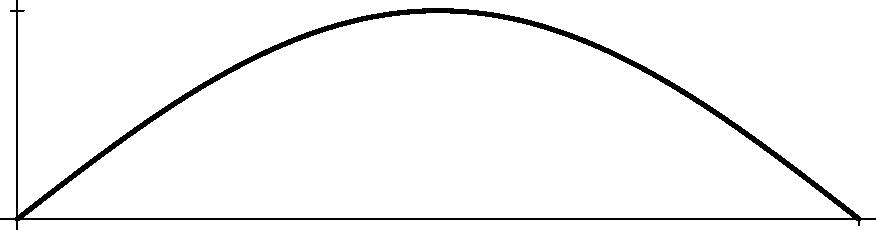
\includegraphics[width=\hsize]{images/e-12}\\
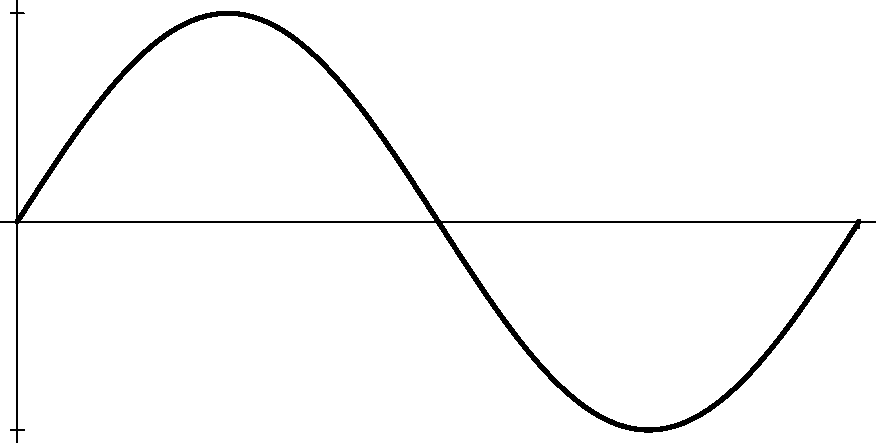
\includegraphics[width=\hsize]{images/e-13}\\
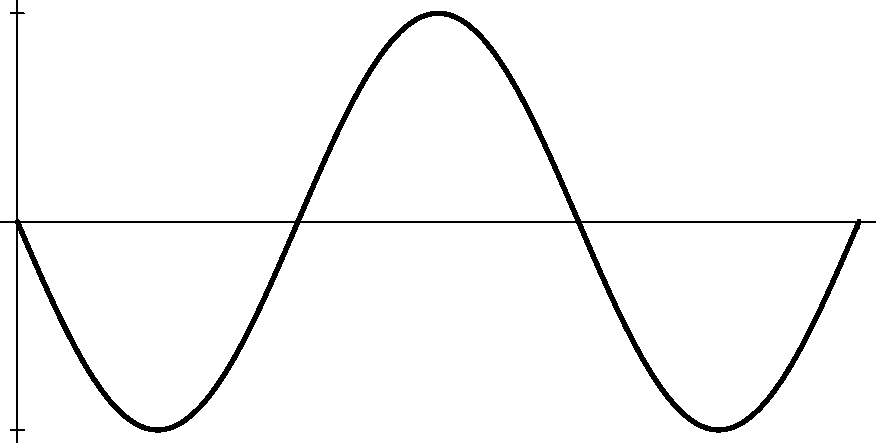
\includegraphics[width=\hsize]{images/e-14}
\end{center}
\caption{Die ersten drei Eigenvektoren einer Federkette mit $n=100$
Massen\label{eigenvektoren-n100}}
\end{figure}
In Abbildung \ref{eigenvektoren-n100} sind die Komponenten der drei
Eigenvektoren mit der geringsten Frequenz dargestellt.
Die "Ahnlichkeit mit den Sinusfunktionen l"asst sich dadurch erkl"aren,
dass die Federkette die diskrete Variante eines kontinuierlichen
Problems ist, n"amlich der Schwingung einer Saite, deren L"osungen
tats"achlich die trigonometrischen Funktionen sind.

\subsection{Fibonacci-Zahlen}
\index{Fibonacci-Folge}
In der Folge der Fibonacci-Zahlen
$$0,1,1,2,3,5,8,13,21,34,55,89,144,\dots$$
entsteht das n"achste Element als Summe der beiden vorangegangenen
Elemente. Die Folge ist offenbar festgelegt, wenn man die zwei ersten
Werte $0$ und $1$ festlegt. Durch Wahl eines anderen Paares von Startzahlen
erh"alt man eine alternative Fibonacci-Folge. Die Fibonacci-Zahlen
erf"ullen die Gleichung 
$$x_{n+1}=x_n+x_{n-1},$$
die wir
auch 
\begin{equation}
x_{n+1}-x_n-x_{n-1}=0
\end{equation}
schreiben k"onnen. Eine solche Gleichung heisst eine Differenzengleichung.

\begin{figure}
\begin{center}
\begin{tabular}{cc}
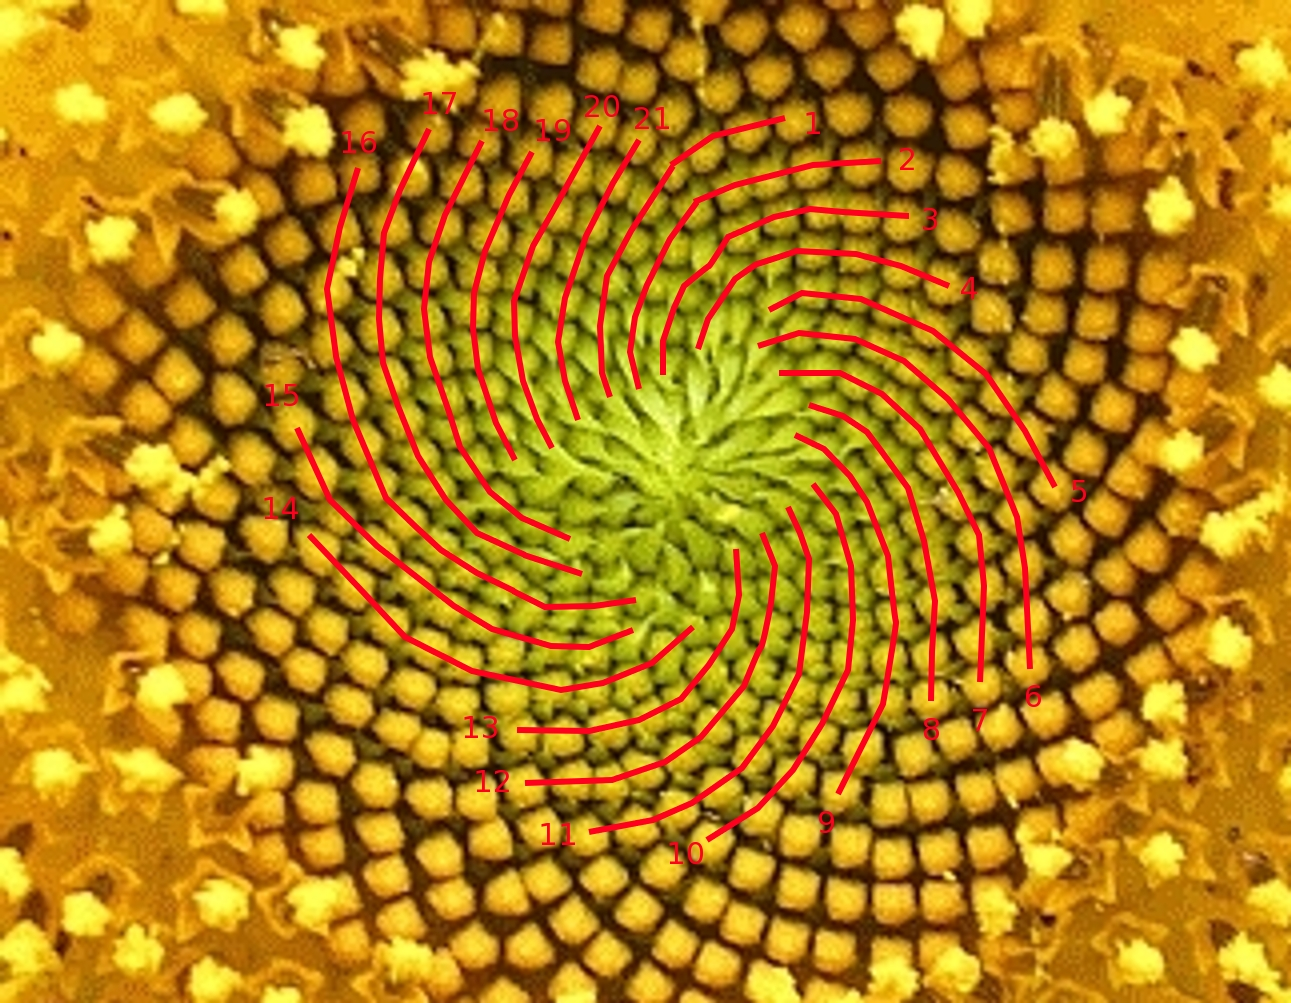
\includegraphics[width=0.47\hsize]{images/helianthus-fibonacci2.jpg}&%
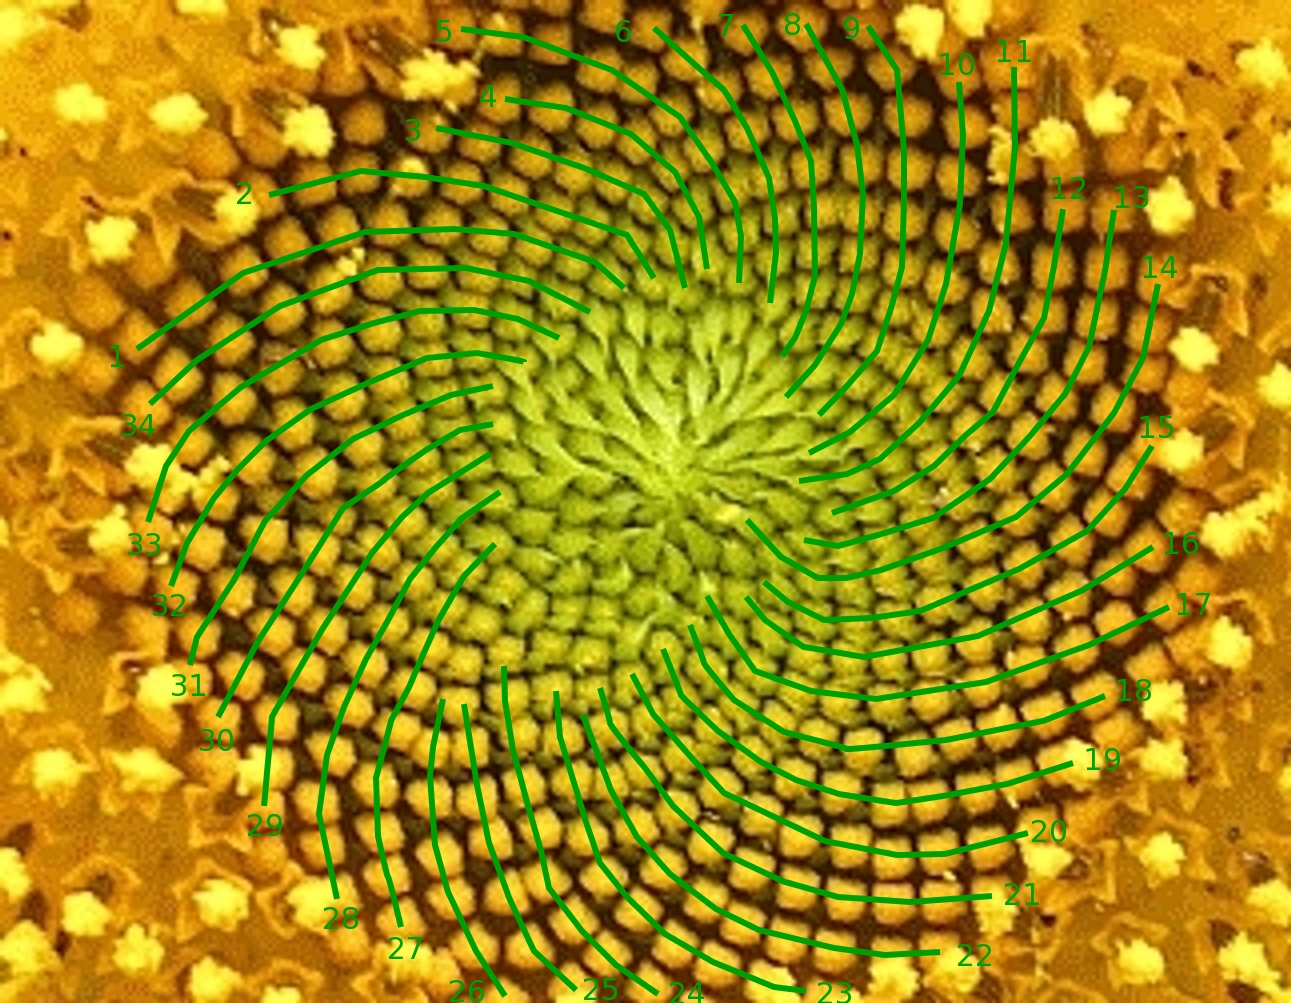
\includegraphics[width=0.47\hsize]{images/helianthus-fibonacci3.jpg}\\%
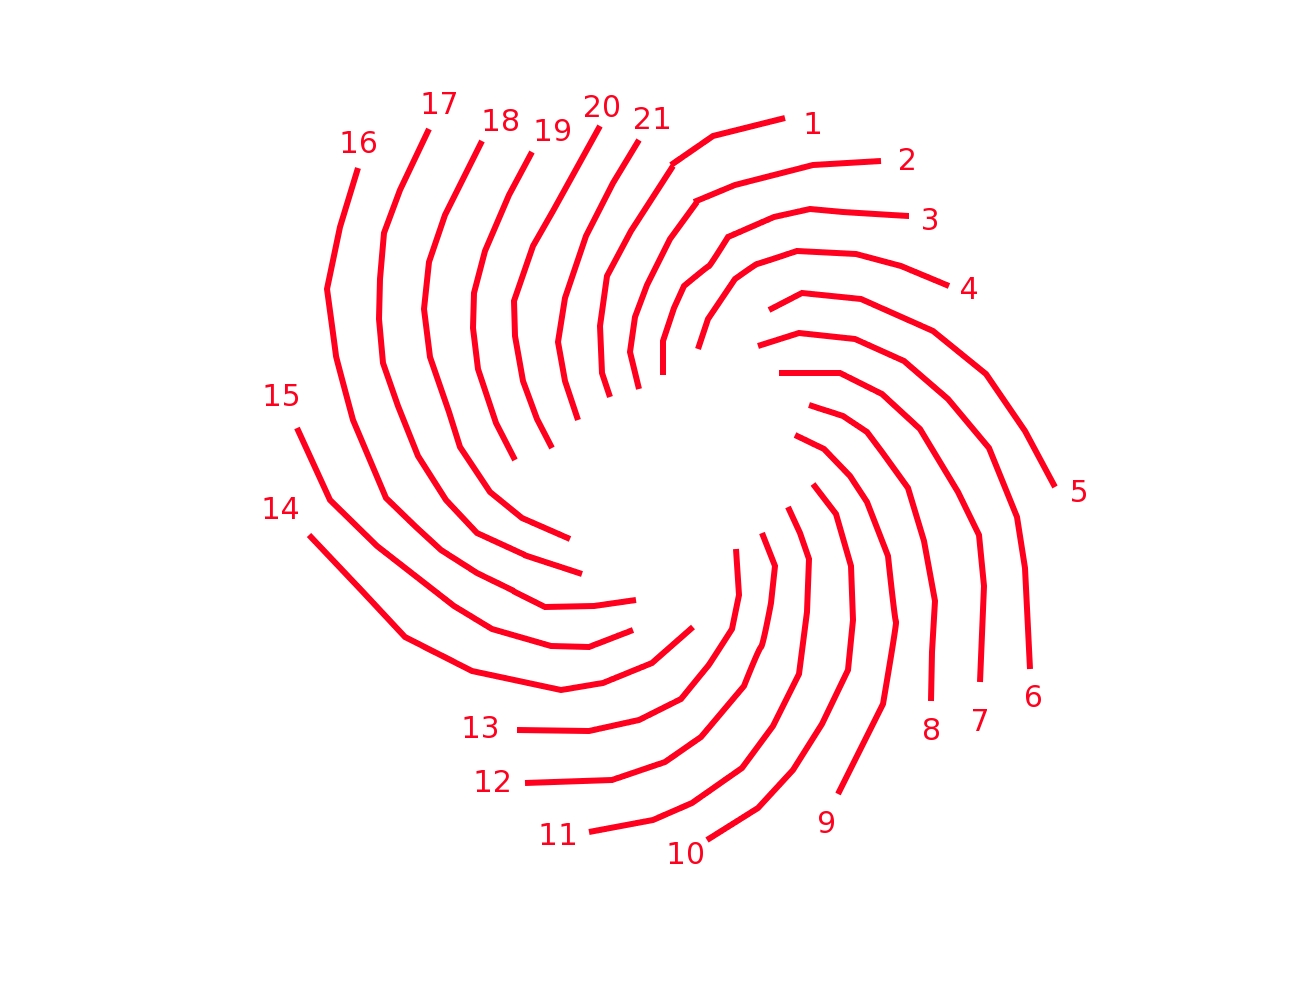
\includegraphics[width=0.47\hsize]{images/helianthus-fibonacci5.jpg}&%
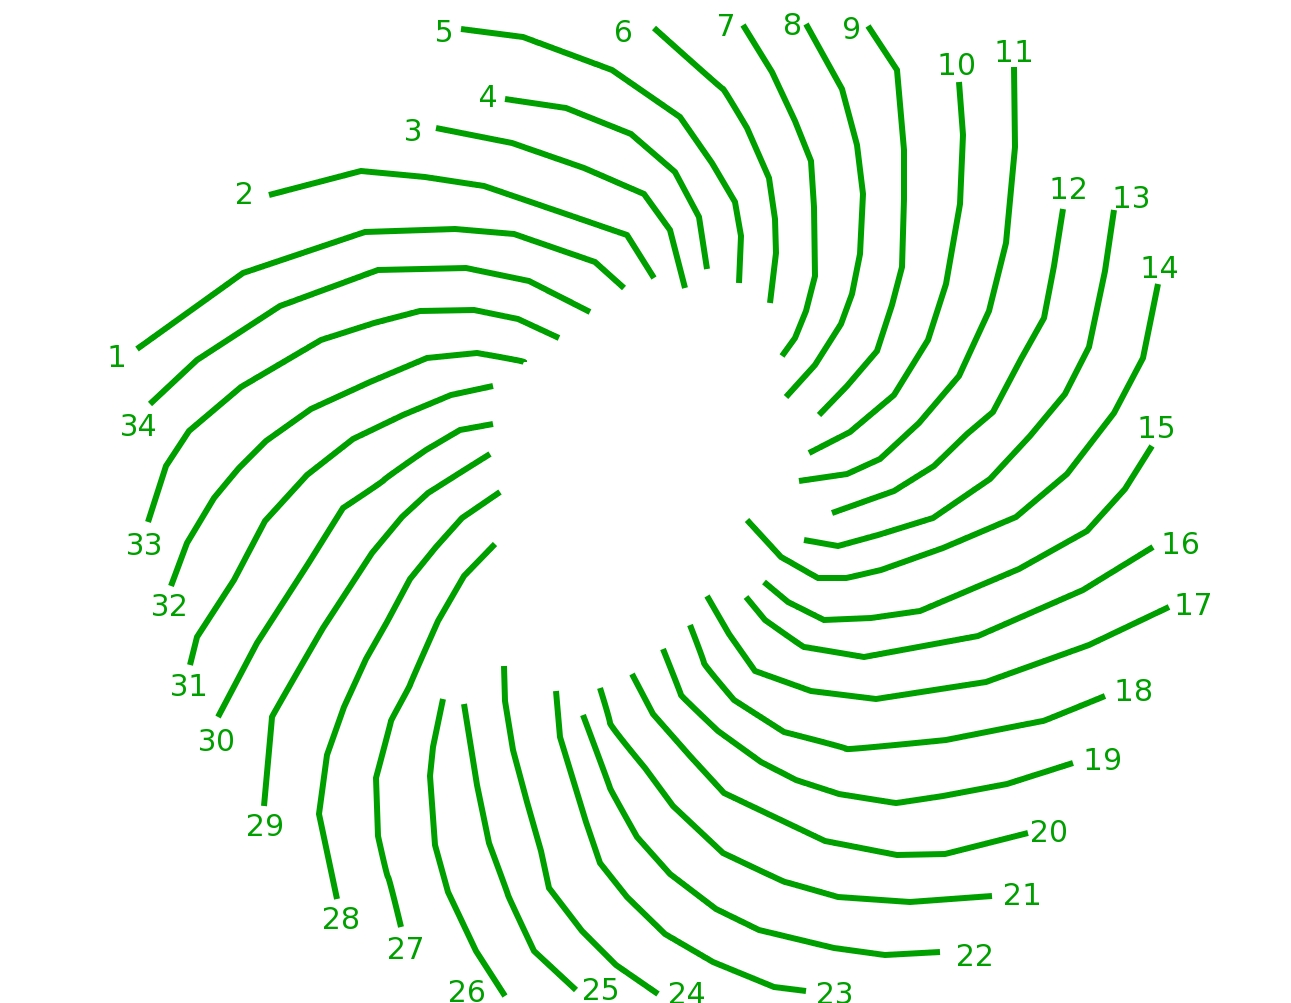
\includegraphics[width=0.47\hsize]{images/helianthus-fibonacci4.jpg}
\end{tabular}
\end{center}
\caption{Die Anzahl der Spiralen in den Bl"utenst"anden von Sonnenblumen
sind aufeinenanderfolgende Fibonacci-Zahlen, hier $21$ (rot) und $34$ (gr"un).
\label{helianthus}}
\end{figure}

Die Fibonacci-Zahlen kommen erstaunlich oft vor:
\begin{itemize}
\index{Sonnenblume}
\index{Tannzapfen}
\index{Ananas}
\index{Romanesco-Broccoli}
\index{goldener Schnitt}
\index{Lateralus}
\item In den Bl"utenst"anden von Sonnenblumen kann man jeweils zwei
Scharen von Spiralen erkennen, auf denen die Sonnenblumenkerne angeordnet sind.
Die Anzahlen der Spiralen in jeder Schar sind jeweils zwei aufeinanderfolgende
Fibonacci-Zahlen (Abbildung~\ref{helianthus}).
\item Auch in Tannzapfen, auf einer Ananas oder auf Romanesco-Broccoli
kann man diese Spiralen erkennen.
\item Das Verh"altnis aufeinanderfolgender Fibonacci-Zahlen strebt gegen
$\frac{1+\sqrt{5}}2$, dem Verh"altnis des goldenen Schnittes, dem schon die
Griechen besondere "asthetische Qualit"aten nachsagten.
\item Im Song `Lateralus' der Gruppe Tool ist die Anzahl der Silben
in jedem Textblock eine Fibonacci-Zahl, und auch der Rythmus basiert
auf den Fibonacci-Zahlen.
\end{itemize}

\subsubsection{Rekursionsgleichung als Matrizengleichung}
\index{Rekursionsgleichung}
Um die Fibonacci-Zahlen zu berechnen, muss man sich nur jeweils die letzten zwei
Zahlen merken, wir schreiben diese in eine Spaltenvektor
$$\begin{pmatrix}x_n\\x_{n-1}\end{pmatrix}$$
Beim "Ubergang zur Fibonacci-Zahl $x_{n+1}$ muss man sich auch $x_n$ merken,
man muss also den neuen Spaltenvektor berechnen:
\begin{equation}
\begin{pmatrix}x_{n+1}\\x_n\end{pmatrix}
=
\begin{pmatrix}x_n+x_{n-1}\\x_n\end{pmatrix}
=
\begin{pmatrix}
1&1\\
1&0
\end{pmatrix}
\begin{pmatrix}x_n\\x_{n-1}\end{pmatrix}
=
A
\begin{pmatrix}x_n\\x_{n-1}\end{pmatrix}
\label{fibonaccirekursion}
\end{equation}
\subsubsection{L"osung als Eigenwertproblem}
Nat"urlich ist es etwas umst"andlich, zum Beispiel die 1291-ste Fibonacci-Zahl
zu berechnen, da w"are eine Formel $f(n)$ sehr praktisch, in der man einfach
die Zahl 1291 einsetzen k"onnte.
Die Fibonacci-Zahlen nehmen sehr schnell zu, 
wir versuchen die L"osung in der Form
$$f(n)=a\lambda^n$$
zu finden. Eingesetzt in (\ref{fibonaccirekursion}) ergibt sich
$$
\begin{pmatrix}a\lambda^{n+1}\\a\lambda^n\end{pmatrix}
=A\begin{pmatrix}a\lambda^n\\a\lambda^{n-1}\end{pmatrix}
$$
Der Vektor auf der linken Seite ist das $\lambda$-fache des Vektors
auf der rechten Seite, wenn es also "uberhaupt eine L"osung in der
Form $f(n)=a\lambda^n$ gibt, dann gibt es auch einen Vektor $y$, der
die Gleichung
\begin{equation}
Ay=\lambda y, \qquad y=\begin{pmatrix}
a\lambda^n\\a\lambda^{n-1}
\end{pmatrix}
\end{equation}
erf"ullt. In diesem Gleichungssystem kommen die Unbekannten auch auf
der rechten Seite vor, die Standard-Form ist daher
$$Ay-\lambda y=(A-\lambda I)y=0.$$
Wir m"ussen also herausfinden, f"ur welche Werte von $\lambda$ dieses
Gleichungssystem "uberhaupt eine nichttriviale L"osung (und damit unendlich
viele L"osungen) hat. Dies geschieht genau dann, wenn die Determinante
der Matrix
$$A-\lambda I=\begin{pmatrix}1-\lambda&1\\1&-\lambda\end{pmatrix}$$
verschwindet. Berechnung der
Determinante ergibt die quadratische Gleichung
$$\det
\begin{pmatrix}1-\lambda&1\\1&-\lambda\end{pmatrix}
=(1-\lambda)(-\lambda)-1=\lambda^2-\lambda-1=0.
$$
Sie hat die L"osungen
$$
\lambda_{\pm}=\frac12+\pm\sqrt{\frac14+1}=\frac{1\pm\sqrt{5}}2.
$$
F"ur jeden Wert $\lambda_{\pm}$ gibt es einen nichttrivialen
L"osungsvektor, den man durch L"osen des Gleichungssystems nach
Einsetzen von $\lambda_{\pm}$ erhalten kann. 

Setzt man $\lambda_+$ ein, bekommt man die Koeffizientenmatrix
$$
A-\lambda_+I=
\begin{pmatrix}
1-\lambda_+&1\\1&-\lambda_+
\end{pmatrix}
=
\begin{pmatrix}
\frac{1-\sqrt{5}}2&1\\1&-\frac{1+\sqrt{5}}2
\end{pmatrix}
$$
Wir wissen bereits, dass das Gleichungssystem $(A-\lambda_+I)y=0$
eine nichttriviale L"osung hat, zum Beispiel
$$y_+=\begin{pmatrix}
\frac{1+\sqrt{5}}2\\1
\end{pmatrix}
=\begin{pmatrix}
\lambda_+\\1
\end{pmatrix}
$$
Analog hat man f"ur $\lambda_-$ die Matrix
$$
A-\lambda_-I=
\begin{pmatrix}
\frac{1+\sqrt{5}}2&1\\
1&-\frac{1-\sqrt{5}}2
\end{pmatrix}
$$
und eine nichttriviale L"osung 
$$y_-=\begin{pmatrix}
\frac{1-\sqrt{5}}2\\
1
\end{pmatrix}=
\begin{pmatrix}
\lambda_-\\1
\end{pmatrix}
$$
\subsubsection{Anfangswerte}
Wir haben inzwischen die Folgen
$$
\begin{matrix}
1&\lambda_+&\lambda_+^2&\lambda_+^3&\lambda_+^4&\dots\\
1&\lambda_-&\lambda_-^2&\lambda_-^3&\lambda_-^4&\dots
\end{matrix}
$$
gefunden, die beide L"osungen des Rekursionsgleichung sind, die Summe
zweier Folgenglieder ergibt das n"achste Glied.
Diese Eigenschaft bleibt auch erhalten, wenn wir zwei beliebige
Vielfache dieser Folgen addieren. Die Folge
$$
\begin{matrix}
A+B
&A\lambda_++B\lambda_-
&A\lambda_+^2+B\lambda_-^2
&A\lambda_+^3+B\lambda_-^3
&\dots
&A\lambda_+^n+B\lambda_-^n
&\dots
\end{matrix}
$$
ist auch eine L"osung der Rekursionsgleichung. Tats"achlich k"onnen
wir die L"osung
$x_n=A\lambda_+^n + B\lambda_-^n$
in die Rekursionsgleichung einsetzen:
\begin{align*}
x_{n+1}-x_n-x_{n-1}
&=A\lambda_+^{n+1} + B\lambda_-^{n+1}
-x_n=A\lambda_+^n - B\lambda_-^n
-x_{n-1}=A\lambda_+^n - B\lambda_-^{n-1}
\\
&=
A(\lambda_+^{n+1}-\lambda_+^n-\lambda_+^{n-1})
+
B(\lambda_-^{n+1}-\lambda_-^n-\lambda_-^{n-1})
\\
&=0
\end{align*}
Die Klammerausdr"ucke verschwinden, weil $\lambda_+^n$ und $\lambda_-^n$
f"ur sich bereits L"osungen der Rekursionsgleichung sind.

Wir m"ochten jetzt eine Folge konstruieren, die mit bestimmten Werten
$0$ und $1$ beginnt, dazu m"ussen wir die Koeffizienten $A$ und $B$
bestimmen:
$$
\begin{matrix}
A\phantom{\lambda_+}&+&B\phantom{\lambda_-}&=&0
\\
A\lambda_+&+&B\lambda_-&=&1
\end{matrix}
$$
Es ist also ein Gleichungssystem mit Matrix
$$
\begin{pmatrix}
1&1\\\lambda_+&\lambda_-
\end{pmatrix}
$$
und den gew"unschten Anfangswerten als rechten Seiten zu l"osen. In diesem
speziellen Fall ist das Determinanten-Verfahren zweckm"assig:
\begin{align*}
A&=\frac{
\left|
\begin{matrix}
0&1\\1&\lambda_-
\end{matrix}
\right|
}{
\left|
\begin{matrix}
1&1\\\lambda_+&\lambda_-
\end{matrix}
\right|
}
=
\frac{-1}{\lambda_--\lambda_+}=-\frac1{-\sqrt{5}}=\frac1{\sqrt{5}}
\\
B&=\frac{
\left|
\begin{matrix}
1&0\\\lambda_+&1
\end{matrix}
\right|
}{
\left|
\begin{matrix}
1&1\\\lambda_+&\lambda_-
\end{matrix}
\right|
}
=
\frac{1}{\lambda_--\lambda_+}=\frac1{-\sqrt{5}}=-\frac1{\sqrt{5}}
\end{align*}
Somit ist die Folge
\begin{equation}
x_n=\frac1{\sqrt{5}}\left(\frac{1+\sqrt{5}}{2}\right)^n
-\frac1{\sqrt{5}}\left(\frac{1-\sqrt{5}}{2}\right)^n
\label{fibonacci}
\end{equation}
die gesuchte geschlossene Formel f"ur die Fibonacci-Zahlen.
Es ist auf den ersten Blick "uberraschend, dass die Formel
(\ref{fibonacci}) f"ur jeden Wert von $n$ einen nat"urliche
Zahl ergibt, obwohl jeder einzelne Summand irrational ist.

Man kann aus (\ref{fibonacci}) auch andere Eigenschaften der
Fibonacci-Zahlen ablesen. Zum Beispiel ist der Quotient
zweier aufeinanderfolgender Fibonacci-Zahlen
\begin{align*}
\frac{x_{n+1}}{x_n}
&=
\frac{A\lambda_+^{n+1}+B\lambda_-^{n+1}}{A\lambda_+^{n}+B\lambda_-^{n}}
=
\lambda_+\frac{1+\displaystyle\frac{B\lambda_-^{n+1}}{A\lambda_+^{n+1}}}{1+\displaystyle\frac{B\lambda_-^n}{A\lambda_+^n}}
=
\lambda_+\frac{1-q^{n+1}}{1-q^n},
\end{align*}
wobei $q=\lambda_+/\lambda_-$. Da $q<1$ ist, werden die Potenzen $q^n$
f"ur grosse $n$ beliebig klein, und damit auch
$$\lim_{n\to\infty}\frac{x_{n+1}}{x_n}=\lambda_+,$$
der Quotient aufeinanderfolgender Fibonacci-Zahlen strebt also gegen
$\lambda_+$.

\subsubsection{Verallgemeinerung}
Das eben dargestellte Verfahren zur L"osung einer endlichen 
Differenzengleichung l"asst sich verallgemeinern.
Eine Differenzengleichung der Form
$$
x_{n+1}=a_kx_n+a_{k-1}x_{n-1}+\dots+a_1x_{n-k+1}+a_0x_{n-k}
$$
kann in vektorieller Form als
$$
\begin{pmatrix}
x_{n-k+1}\\
x_{n-k+2}\\
\vdots\\
x_{n}\\
x_{n+1}
\end{pmatrix}
=
\begin{pmatrix}
0&1&0&\dots&0\\
0&0&1&\dots&0\\
\vdots&\vdots&\vdots&\ddots&\vdots\\
0&0&0&\dots&1\\
a_0&a_1&a_2&\dots&a_k
\end{pmatrix}
\begin{pmatrix}
x_{n-k}\\
x_{n-k+1}\\
\vdots\\
x_{n-1}\\
x_n
\end{pmatrix}
$$
geschrieben werden, wir bezeichnen die $k\times k$-Matrix mit $A$. 
Mit einem Ansatz der Form $x_n=\lambda^n$ und
$$
x=
\begin{pmatrix}
\lambda^{n-k}\\
\vdots\\
\lambda^n
\end{pmatrix}
$$
wird daraus ein
Eigenwert-Problem
$$
\begin{pmatrix}
\lambda_{n-k+1}\\
\vdots\\
\lambda^{n+1}
\end{pmatrix}
=
\lambda x
=A
\begin{pmatrix}
\lambda^{n-k}\\
\vdots\\
\lambda^n
\end{pmatrix}
=Ax
$$
Im allgemeinen wird es $k$ verschiedene Werte $\lambda_1,\dots\lambda_k$ geben,
f"ur die dieses Gleichungssystem eine nichtriviale L"osung hat.
Eine Linearkombination der L"osungen $\lambda_i^n$ ist wiederum eine
L"osung der Differenzengleichung. Sogar die Wachstumseigenschaft l"asst
sich verallgemeinern: der Quotient aufeinanderfolgender Folgenglieder
einer L"osung strebt gegen den betragsm"assig gr"ossten Eigenwert $\lambda_i$
unter den zur L"osung kombinierten $\lambda_i^n$.

\section{Charakteristische Gleichung}
\index{charakteristische Gleichung}
Welche Eigenwerte und Eigenvektoren hat eine Matrix? Ein Eigenvektor 
ist ein von $0$ verschiedener Vektor $x$, der die Gleichung
$Ax=\lambda x$ erf"ullt, oder wie wir fr"uher gesehen haben,
eine nicht verschwindende L"osung des homogenen Gleichungssystems
$(A-\lambda E)x=0$.
Im Kapitel \ref{chapter-determinanten} wurde gezeigt, dass ein eine solche
L"osung nur dann existieren kann, wenn die Determinante des Gleichungssystems
verschwindet, also
$$\det(A-\lambda E)=
\left|
\begin{matrix}
a_{11}-\lambda&a_{12}&\dots&a_{1n}\\
a_{21}&a_{22}-\lambda&\dots&a_{2n}\\
\vdots&\vdots&\ddots&\vdots\\
a_{n1}&a_{n2}&\dots&a_{nn}-\lambda
\end{matrix}
\right|
$$
Die Determinante ist ein Polynom $n$-ten Grades in $\lambda$, das Finden der
Eigenwerte l"auf also darauf hinaus, Nullstellen eines Polynoms zu finden.
\begin{satz}
Die Eigenwerte einer $n\times n$ Matrix $A$ sind Nullstellen des
Polynoms
$$
\chi_A(\lambda)=\det(A-\lambda E)
$$
vom Grad $n$.
\end{satz}
\begin{definition}
\index{charakteristisches Polynom}
Das Polynom $\chi_A(\lambda)=\det(A-\lambda E)$ heisst
charakteristisches Polynom,
die Gleichung $\chi_A(\lambda)=0$ heisst 
charakteristische Gleichung.
\end{definition}

\begin{beispiel}
Die Matrix $A=\begin{pmatrix}0&1\\1&0\end{pmatrix}$ hat das 
charakteristische Polynom
\begin{align*}
\det(A-\lambda I)&=\left|\begin{matrix}-\lambda&1\\1&-\lambda\end{matrix}\right|\\
&=\lambda^2-1=(\lambda+1)(\lambda-1)
\end{align*}
mit den L"osungen $\lambda_\pm=\pm1$. Um die Eigenvektoren zu finden, muss
man jetzt das Gleichungssystem $(A-\lambda E)x=0$ bestimmen. F"ur die Eigenwerte
$\pm1$ hat das Gleichungssystem die Matrizen
\[
\begin{pmatrix}
-1&1\\1&-1
\end{pmatrix}\quad \text{f"ur $\lambda=1$},\qquad
\begin{pmatrix}
1&1\\1&1
\end{pmatrix}\quad\text{f"ur $\lambda=-1$}
\]
mit den L"osungsvektoren 
\[
\vec v_+=\begin{pmatrix}1\\1\end{pmatrix},
\qquad
\vec v_-=\begin{pmatrix}1\\-1\end{pmatrix}.
\]
\end{beispiel}

\section{Diagonalisierung symmetrischer Matrizen\label{section-diag-sym}}
\index{Matrix!symmetrische}
Falls eine Basis aus Eigenvektoren existiert, l"asst sich eine Matrix
besonders einfach als Diagonalmatrix darstellen. Leider ist die Existenz
einer Basis aus Eigenvektoren im Allgemeinen nicht garantiert, und noch
viel weniger darf man annehmen, dass eine orthonormierte Basis
von Eigenvektoren existiert. Im Spezialfall einer symmetrischen Matrix
ist dies jedoch immer m"oglich, wie in diesem Abschnitt gezeigt werden
soll.

In diesem Abschnitt sei $A$ eine symmetrische $n\times n$-Matrix,
also  $A^t=A$.

\begin{hilfssatz}
Sind $v_1$ und $v_2$ Eigenvektoren von $A$ zu den Eigenwerten 
$\lambda_1$ und $\lambda_2$ mit $\lambda_1\ne \lambda_2$, dann
ist $v_1\cdot v_2=0$.
\end{hilfssatz}

\begin{proof}[Beweis]
Wir berechnent das Skalarprodukt $v_1\cdot Av_2$ auf zwei verschiedene
Arten, wobei wir in der zweiten Variante ausn"utzen, dass $A=A^t$:
\begin{align*}
v_1^tAv_2&=\lambda_2v_1^tv_2
\\
v_1^tAv_2&=v_1^tA^tv_2=(Av_1)^tv_2=\lambda_1v_1^tv_2
\\
\Rightarrow
\qquad
0&=(\lambda_2-\lambda_1)v_1^tv_2
\end{align*}
Da $\lambda_2\ne\lambda_1$ ist $\lambda_2-\lambda_1\ne 0$, man kann
also durch den Klammerausdruck teilen und findet
$$v_1^tv_2=v_1\cdot v_2=0,$$
die beiden Eigenvektoren stehen also senkrecht aufeinander.
\end{proof}

\begin{hilfssatz}
\label{ev-ortho}
Ist $v$ ein Eigenvektor zum Eigenwert $\lambda$, und $w\perp v$ ein weiterer
Vektor, dann ist auch $Aw\perp v$.
\end{hilfssatz}

\begin{proof}[Beweis]
Wir berechnen das Skalarprodukt
$$
(Aw)\cdot v=(Aw)^t v=w^tA^tv=w^tAv=w^t\lambda v=\lambda w\cdot v=0,
$$
also $Aw\perp v$.
\end{proof}

\begin{hilfssatz}
\label{ev-existenz}
Sei $v$ ein Einheitsvektor f"ur den $v^tAv$ den minimalen Wert $\lambda$ annimmt.
Dann ist $v$ ein Eigenvektor zum Eigenwert $\lambda$.
\end{hilfssatz}

\begin{proof}[Beweis]
Wir m"ussen zeigen, dass $Av=\lambda v$. Da $v$ so gew"ahlt war, dass
$v^tAv$ minimal wird, berechnen wir 
\begin{align*}
f(t)&=\frac{(v+ty)^tA(v+ty)}{(v+ty)^t(v+ty)}
\\
&=
\frac{v^tAv+t(y^tAv+v^tAy)+t^2y^tAy}{v^tv+t(y^tv+v^ty)+t^2v^tv}
\\
f'(0)
&=
\frac{ (y^tAv+v^tAy)v^tv + v^tAv(y^tv+v^ty) }{ (v^tv)^2 }
\\
&=
\frac{ (y^tAv+v^tAy) - \lambda (y^tv+v^ty) }{ v^tv }
\\
&=
2\frac{ v^tAy - \lambda v^ty }{ v^tv }
\\
&=
2\frac{ (Av - \lambda v)^ty }{ v^tv }=0
\end{align*}
Da dies f"ur jeden Vektor $y$ gilt, folgt $Av-\lambda v=0$, also
$Av=\lambda v$, $v$ ist also ein Eigenvektor.
\end{proof}

\begin{satz}
\label{satz:symmetrischdiagonalisierbar}
Sei $A$ eine symmetrische Matrix, dann gibt es eine orthonormierte Basis
von Eigenvektoren von $A$.
\end{satz}

\begin{proof}[Beweis]
Wir beweisen diesen Satz mit Induktion nach der Dimension des Vektorraumes.

Ein $1$-dimensionaler Raum enth"alt ausschliesslich Eigenvektoren.

Sei jetzt also ein Vektorraum der Dimension $n$.
Nach Hilfssatz \ref{ev-existenz} gibt es mindestens einen Eigenvektor $v_1$
zum Eigenwert $\lambda$.  Die Menge der Vektoren, die auf $v_1$ senkrecht
stehen, bilden einen Vektorraum $V_1$. Die durch $A$ definierte Abbildung
bildet Vektoren aus $V_1$ nach Hilfssatz \ref{ev-ortho} wieder nach
$V_1$ ab. Die Dimension von $V_1$ ist um $1$ kleiner, nach der
Induktionsannahme gibt es also ein Basis von Einheitsvektoren in $V_1$.
Damit ist auch in $V$ eine Basis aus Eigenvektoren konstruiert.
\end{proof}

\begin{beispiel} Eine symmetrische $2\times 2$-Matrix 
\[
A=\begin{pmatrix}a&b\\b&c\end{pmatrix}
\]
ist nach Satz \ref{satz:symmetrischdiagonalisierbar} diagonalisierbar.
Unter welchen Bedingungen haben die beiden Eigenwerte das gleiche
oder verschiedenes Vorzeichen?

\smallskip
{\parindent 0pt Die Eigenwerte k"onnen mit dem charakteristischen
Polynom berechnet werden:}
\[
\left|\;
\begin{matrix}a-\lambda & b\\ b&c-\lambda\end{matrix}
\;\right|=(a-\lambda)(c-\lambda)-b^2
=
\lambda^2-(a+c)\lambda+ ac-b^2=0
\]
Die zwei Eigenwerte $\lambda_1$ und $\lambda_2$ sind Nullstellen
dieses Polynoms, also gilt
\begin{align*}
(\lambda-\lambda_1)(\lambda-\lambda_2)&=\lambda^2-(\lambda_1+\lambda_2)\lambda
+\lambda_1\lambda_2=
\lambda^2-(a+c)\lambda+ ac-b^2=0\\
\Rightarrow\qquad
\lambda_1+\lambda_2&=a+c\\
\lambda_1\lambda_2&=ac-b^2
\end{align*}
Wir w"ahlen die Bezeichnungen so, dass $\lambda_1$ der gr"ossere Eigenwert ist.
Haben beide Eigenwerte das gleiche Vorzeichen, ist $ac-b^2>0$. In diesem
Fall kann man das gemeinsame Vorzeichen der Eigenwerte an der Summe
$\lambda_1+\lambda_2=a+c$ ablesen. Die Resultate sind in Tabelle
\ref{vorzeichen-eigenwerte} zusammengestellt.
\begin{table}
\begin{center}
\begin{tabular}{|>{$}c<{$}|>{$}c<{$}|>{$}c<{$}|>{$}c<{$}|}
\hline
	&a+c\ge0
		&a+c\le0
\\
\hline
ac-b^2>0
	&\lambda_1\ge\lambda_2>0
		&\lambda_2\le\lambda_1<0
\\
\hline
ac-b^2=0
	&\lambda_1\ge 0
		&\lambda_1=0
\\
	&\lambda_2=0
		&\lambda_2 \le 0
\\
\hline
ac-b^2<0
	&\lambda_1>0
		&\lambda_1>0
\\
	&\lambda_2<0
		&\lambda_2<0
\\
	&\lambda_1\ge|\lambda_2|
		&\lambda_1\le|\lambda_2|
\\
\hline
\end{tabular}
\end{center}
\caption{Vorzeichen und relative Gr"osse der Eigenwerte einer
symmetrischen $2\times 2$-Matrix
\label{vorzeichen-eigenwerte}}
\end{table}
\end{beispiel}

\begin{beispiel}[Zahlenbeispiel]
Welche Vorzeichen haben die Eigenwerte der symmetrische Matrix
\[
A=\begin{pmatrix}
3&4\\
4&5
\end{pmatrix}?
\]

\smallskip
{\parindent 0pt $\det(A)=-1$ und $3+5=8>0$, also kann man aus der
Tabelle \ref{vorzeichen-eigenwerte}
ablesen, dass die beiden Eigenwerte entgegengesetztes
Vorzeichen haben, und dass der negative Eigenwert betragsm"assig
kleiner ist.}

Man kann die Eigenwerte nat"urlich auch ausrechnen. Die charakteristische
Gleichung ist 
\[
\lambda^2-8\lambda-1=0
\]
und hat die L"osungen
\[
\lambda_{1,2}=4\pm\sqrt{16+1}=\begin{cases}
4+\sqrt{17}&=\phantom{-}8.12311\\
4-\sqrt{17}&=-0.12311
\end{cases}
\]
Dies best"atigt die aus der Tabelle abgeleiteten Schl"usse.
\end{beispiel}

\section{Numerische L"osung des Eigenwertproblems}
In der Praxis m"ussen meist grosse Eigenwertprobleme gel"ost werden.
Das Vorgehen "uber das charakteristische Polynom ist dabei nicht zweckm"assig,
einerseits ist es sehr aufwendig zu berechnen, andereseits ist die
Berechnung der Nullstellen eines Polynoms hohen Grades mit dem Computer
keineswegs einfach.

Ein f"ur praktische Anwendungen besonders wichtiger Fall ist
das Eigenwertproblem f"ur symmetrische Matrizen.
Aus Abschnitt \ref{section-diag-sym} wissen wir, dass sich symmetrische
Matrizen sogar mit einer orthonormierten Basis diagonalisieren lassen.
Es muss also eine orthogonale Matrix $T$ geben, welche $A$ auf
Diagonalform transformiert, oder $T^tAT$ muss diagonal sein.
Oder $A=TDT^t$, mit einer Diagonalmatrix $D$.
Die in Abschnitt \ref{section-svd} beschriebene Singul"arwertzerlegung
liefert genau so eine Zerlegung der Matrix, die Matrix $S$ von 
Satz \ref{satz-svd} ist also die gesuchte Diagonalmatrix, die
Singul"arwerte sind die Eigenwerte, und die Transformationsmatrix
entspricht den Matrizen $U$ und $V$, die in diesem Falle gleich sind:
$T=U=V$. 

Die Singul"arwertzerlegung ist tats"achlich die Basis vieler Implementation
von Algorithmen zur Bestimmung der Eigenwerte und Eigenvektoren. 
Octave/Matlab hat aber auch eine eigene Funktion zur Berechnung der
Eigenwerte und Eigenvektoren.
\begin{beispiel}
Es sollen die Eigenwerte und Eigenvektoren der Matrix
\[
A=\begin{pmatrix}0&1\\1&0\end{pmatrix}
\]
bestimmt werden.

Die Eigenwerte sind der R"uckgabewert der Funktion {\tt eig}:
\begin{verbatim}
6> eig([0,1;1,0])
ans =

  -1
   1
\end{verbatim}
Wenn man aber auch die Eigenvektoren braucht, muss man als R"uckgabewert
einen Vektor anfordern:
\begin{verbatim}
> [T, D] = eig([0,1;1,0])
T =

  -0.70711   0.70711
   0.70711   0.70711

D =

Diagonal Matrix

  -1   0
   0   1
\end{verbatim}
In den Spalten der Matrix $T$ stehen die Eigenvektoren, es ist
$D=T^{-1}AT$, wie man auch mit Octave nachrechnen kann:
\begin{verbatim}
0> T^-1 * A * T
ans =

  -1   0
   0   1
\end{verbatim}
Die Matrix $T$ enth"alt also als Spalten genau die Eigenvektoren,
also die Vektoren einer Basis, in der $A$ diagonal wird.
\end{beispiel}
Die n"achsten Abschnitte sollen jetzt aber die Frage beantworten,
wie ein solches Verfahren funktionieren kann.

\subsection{Jacobi-Verfahren}
\index{Eigenwertberechnung!mit dem Jacobi-Algorithmus}
\index{Jacobi, Carl Gustav}
\index{Jacobi-Algorithmus}
Ein einfach zu verstehender Algorithmus zur Bestimmung der Eigenwerte
ist der Jacobi-Algorithmus. Er bestimmt eine angen"aherte Matrix
$T$ iterativ. Man erh"alt also nicht wie bei Gauss-Algorithmus und
den Matrixzerlegungen direkt eine exakte L"osung, sondern nur eine
mehr oder weniger gute N"aherungsl"osung, die durch weitere Iterationen
verbessert werden kann.

Die Idee ist, die Matrix $T$ aus Drehmatrizen in einer der Koordinaten-Ebenen
zusammenzusetzen. Die Drehung um den Winkel $\alpha$ in der Ebene
$x_i$-$x_k$-Ebene hat die Matrix
\begin{equation}
D_{\alpha,i,k}=\begin{pmatrix}
1     &      &           &      &           &      &      \\
      &\ddots&           &      &           &      &      \\
      &      & \cos\alpha&      &-\sin\alpha&      &      \\
      &      &           &\ddots&           &      &      \\
      &      & \sin\alpha&      & \cos\alpha&      &      \\
      &      &           &      &           &\ddots&      \\
      &      &           &      &           &      &1     \\
\end{pmatrix}
\label{matrixd}
\end{equation}
die nat"urlich orthogonal ist.
Diese Drehungen heissen Givens-Rotationen.
\index{Givens-Rotation}
Ausserdem ist
$D_{\alpha,i,k}^{-1}=D_{-\alpha,i,k}$. Jetzt versucht man mit
einer solchen Drehmatrix aus $A$ eine Matrix zu machen, die 
eher wie eine Diagonalmatrix aussieht. Nat"urlich geht das
normalerweise nicht exakt, aber man kann wenigstens fordern,
dass in $A''= D^{-1}AD=D^tAD$ die Elemente $a''_{ik}=0$ sind.

Wir f"uhren jetzt die Berechnung des Produktes durch.
Zun"achst das Produkt $A'=AD$,
\[
A'
=
\begin{pmatrix}
a_{11}&\dots &a_{1i}\cos\alpha - a_{1k}\sin\alpha
		&\dots  & a_{1i}\sin\alpha+a_{1k}\cos\alpha
				&\dots	&a_{1n}\\
\vdots&      &\vdots
		&	&\vdots
				&	&\vdots\\
a_{i1}&\dots &a_{ii}\cos\alpha - a_{ik}\sin\alpha
		&\dots  & a_{ii}\sin\alpha+a_{ik}\cos\alpha
				&\dots	&a_{in}\\
\vdots&      &\vdots
		&	&\vdots
				&	&\vdots\\
a_{k1}&\dots &a_{ki}\cos\alpha - a_{kk}\sin\alpha
		&\dots  & a_{ki}\sin\alpha+a_{kk}\cos\alpha
				&\dots	&a_{kn}\\
\vdots&      &\vdots
		&	&\vdots
				&	&\vdots\\
a_{n1}&\dots &a_{1i}\cos\alpha - a_{1k}\sin\alpha
		&\dots  & a_{1i}\sin\alpha+a_{1k}\cos\alpha
				&\dots	&a_{nn}\\
\end{pmatrix}
\]
Es werden also nur die Elemente in den Spalten $i$ und $k$
ver"andert, und zwar gilt
\begin{equation}
\begin{aligned}
a'_{ji}&=-a_{ji}\cos\alpha-a_{jk}\sin\alpha,\\
a'_{jk}&=-a_{ji}\sin\alpha+a_{jk}\cos\alpha.
\end{aligned}
\label{dtad1}
\end{equation}
Jetzt muss noch von links mit der Matrix $D^t$
multipliziert werden, um $A''=D^tAD=D^tA'$ zu bekommen.
Dabei werden die Zeilen $i$ und $k$ modifiziert.
Die Elemente ausserhalb der Spalten $i$ und $k$ werden 
dabei zu
\begin{equation}
\begin{aligned}
a''_{ij}&=a_{ij}\cos\alpha+a_{kj}\sin\alpha,\\
a''_{kj}&=-a_{ij}\sin\alpha+a_{kj}\cos\alpha.
\end{aligned}
\label{dtad2}
\end{equation}
Die Elemente in den Spalten und Zeilen $i$ und $k$ werden
auch bei diesem zweiten Schritt abege"andert zu
\begin{equation}
\begin{aligned}
a''_{ii}&=\cos\alpha \cdot a'_{ii}+\sin\alpha \cdot a'_{ki}\\
        &=\cos\alpha\cdot (a_{ii}\cos\alpha+a_{ik}\sin\alpha)
         +\sin\alpha\cdot (a_{ki}\cos\alpha+a_{kk}\sin\alpha)\\
        &=a_{ii}\cos^2\alpha-a_{kk}\sin^2\alpha+2a_{ki}\sin\alpha\cos\alpha
\\
a''_{ki}&=-\sin\alpha \cdot a'_{ii}+\cos\alpha \cdot a'_{ki}\\
        &=-\sin\alpha\cdot (a_{ii}\cos\alpha+a_{ik}\sin\alpha)
         +\cos\alpha\cdot (a_{ki}\cos\alpha+a_{kk}\sin\alpha)\\
        &=-\sin\alpha\cos\alpha(a_{ii}-a_{kk})
        +(-\sin^2\alpha+\cos^2\alpha)a_{ki}
\\
a''_{ik}&=\cos\alpha \cdot a'_{ik} +\sin\alpha \cdot a'_{kk}\\
        &=-\cos\alpha\cdot (a_{ii}\sin\alpha+a_{ik}\cos\alpha)
         +\sin\alpha\cdot (-a_{ki}\sin\alpha+a_{kk}\cos\alpha)\\
        &=-\sin\alpha\cos\alpha(a_{ii}-a_{kk})
        +(-\sin^2\alpha+\cos^2\alpha)a_{ik}
\\
a''_{kk}&=-\sin\alpha \cdot a'_{ik}+\cos\alpha \cdot a'_{kk}\\
        &=-\sin\alpha\cdot (-a_{ii}\sin\alpha+a_{ik}\cos\alpha)
         +\cos\alpha\cdot (-a_{ki}\sin\alpha+a_{kk}\cos\alpha)\\
        &=a_{kk}\cos^2\alpha+a_{ii}\sin^2\alpha-2a_{ik}\sin\alpha\cos\alpha
\end{aligned}
\label{dtad3}
\end{equation}
Jetzt muss $\alpha$ so gew"ahlt werden, dass $a''_{ik}=a''_{ki}=0$
wird:
\[
-\sin\alpha\cos\alpha(a_{ii}-a_{kk}) +(-\sin^2\alpha+\cos^2\alpha)a_{ik}=0.
\]
Darin erkennen wir die Doppelwinkelformeln:
\[
-\frac{a_{kk}-a_{ii}}2 \sin2\alpha +a_{ik}\cos2\alpha=0.
\]
Folglich gilt 
\begin{equation}
\tan2\alpha=\frac{2a_{ik}}{a_{ii}-a_{kk}}.
\label{tan2alpha1}
\end{equation}
\index{Halbwinkel-Formel}
Mit der Halbwinkel-Formel f"ur den Tangens bekommt man 
\begin{equation}
\tan\alpha=\frac{\tan2\alpha}{1+\sqrt{1+\tan^22\alpha}}
\label{tan2alpha2}
\end{equation}
und daraus
\begin{align}
\sin\alpha
&=
\frac{\tan\alpha}{\sqrt{1+\tan^2\alpha}},
\\
\cos\alpha
&=
\frac{1}{\sqrt{1+\tan^2\alpha}}.
\label{tan2alpha3}
\end{align}
Insbesondere kann man die Matrix $D$ berechnen, ohne trigonometrische
Funktionen invertieren zu m"ussen, 

Der Algorithmus zur Diagonalisierung von $A$ l"auft jetzt also
wie folgt ab:
\begin{enumerate}
\item Initialisiere $T=E$
\item W"ahle ein Element $a_{ik}\ne 0$, mit $i\ne k$, welches als
n"achstes zu $0$ gemacht werden soll.
\item Bestimme $\tan2\alpha$, $\tan\alpha$, $\sin\alpha$ und $\cos\alpha$
mit den Formeln (\ref{tan2alpha1}) bis (\ref{tan2alpha3}).
\item Bestimme die Matrix $D$ mit Formel (\ref{matrixd}).
\item Bestimme die Matrix $A''$ mit den Formeln (\ref{dtad1}) bis
(\ref{dtad3}).
\item Ersetze $T$ durch $TD$, $A$ durch $A''$.
\item Falls ein Ausserdiagonalelement betragsm"assig $>\varepsilon$,
verwende dessen Zeile $i$ und $k$ und fahre weiter bei Schritt 3.
\end{enumerate}
Dieser Algorithmus terminiert, wenn alle Ausserdiagonalelemente 
betragsm"assig $<\varepsilon$ sind. "Ubrig bleibt in der Matrix
die Diagonalmatrix, mit den Eigenwerten auf der Diagonalen, 
und die Matrix $T$, welche die Eigenschaft hat, dass $T^tAT$
eine Diagonalmatrix ist. Die Eigenvektoren stehen in den
Spalten der Matrix $T$.

\subsection{Potenzmethode\label{section:potenzmethode}}
\index{Potenz-Methode}
F"ur den Spezialfall, dass alle Eigenwerte einer Matrix verschieden
sind, kann man ein relativ simples L"osungsverfahren angeben. In diesem
Abschnitt sei also $A$ eine symmetrische $n\times n$-Matrix mit
verschiedenen Eigenwerten.
\subsubsection{Eigenvektoren zum dominanten Eigenwert\label{section:dominant}}
\index{Eigenwert!dominant}
Nehmen wir an, die Eigenwerte von $A$
seien der Gr"osse nach geordnet:
\[
|\lambda_1| > |\lambda_2| > \dots > |\lambda_n|.
\]
Seien $v_1,\dots,v_n$ die zugeh"origen Eigenvektoren. Jetzt nehmen wir
einen beliebigen Vektor $u$. Da die Eigenvektoren eine Basis bilden,
kann man $u$ in dieser Basis schreiben:
\[
u=u_1v_1+u_2v_2+\dots+u_nv_n.
\]
Wenden wir auf diesen Vektor die Matrix $A$ mehrmals an, entstehen
nacheinander
\begin{align}
Au&=
u_1\lambda_1v_1+u_2\lambda_2v_2+\dots+u_n\lambda_nv_n
\notag
\\
A^2u&=
u_1\lambda_1^2v_1+u_2\lambda_2^2v_2+\dots+u_n\lambda_n^2v_n
\notag
\\
&\vdots
\\
A^ku&=
u_1\lambda_1^kv_1+u_2\lambda_2^kv_2+\dots+u_n\lambda_n^kv_n
\label{power-method-vectors}
\end{align}
Je nach der Gr"osse von $\lambda_i$ wachsen dabei die einzelnen
Terme $u_i\lambda_i^kv_i$ "uber alle Grenzen (wenn $|\lambda_i|>1$)
oder konvergieren gegen $0$ (wenn $|\lambda_i|<1$). Auf jeden Fall
aber wird der erste Term entweder am schnellsten wachsen (wenn $|\lambda_i|>1$)
oder am langsamsten gegen $0$ gehen (wenn $|\lambda_i|<1$). Wenn wir
also den Vektor $A^ku$ immer wieder auf L"ange $1$ normieren, 
werden im Vergleich zum ersten Term alle anderen Terme gegen $0$ gehen.

\begin{beispiel}
Wir betrachten die Matrix 
\[
A=\begin{pmatrix}
1&2&3\\
2&4&5\\
3&5&6
\end{pmatrix}
\]
Die Eigenwerte sind tats"achlich sehr verschieden, Octave findet
die folgenden Werte:
\begin{verbatim}
> eig(A)
ans =

   -0.51573
    0.17092
   11.34481
\end{verbatim}
Jetzt w"ahlen wir einen zuf"alligen Vektor
\begin{verbatim}
5> v = rand(3,1)
v =

   0.12634
   0.68662
   0.56531
\end{verbatim}
und wenden die Matrix $A$ wiederholt darauf an, und normieren nach
jedem Schritt sofort wieder:
\[
v_0 = v,\qquad v_{k+1}=\frac{Av_k}{|Av_k|},\; k\ge 0,
\]
in Octave kann man das durch die Befehle
\begin{verbatim}
> v3 = A * v2; v3 = v3 / norm(v3);
\end{verbatim}
erreichen.
Numerisch erhalten wir Resultate:
\[
v_1=\begin{pmatrix}
   0.32606\\
   0.59444\\
   0.73507
\end{pmatrix}
,\quad
v_2=\begin{pmatrix}
   0.32792\\
   0.59104\\
   0.73698
\end{pmatrix}
,\quad
v_3=\begin{pmatrix}
   0.32799\\
   0.59101\\
   0.73697
\end{pmatrix}
,\quad
v_4=\begin{pmatrix}
   0.32799\\
   0.59101\\
   0.73698
\end{pmatrix}
%,\quad
%v_5=\begin{pmatrix}
%   0.32799\\
%   0.59101\\
%   0.73698
%\end{pmatrix}
\]
Bei $v_5$ ist bereits keine "Anderung mehr feststellbar. Damit
ist der Eigenvektor zum gr"ossten Eigenwert gefunden, 
\end{beispiel}

\subsubsection{Weitere Eigenvektoren}
Hat man einen ersten Eigenvektor $v_1$ gefunden,
kann man das Problem verkleinern.
Die weiteren Eigenvektoren von $A$ stehen ja alle auf  $v_1$
senkrecht. Man kann also eine Basistransformation
durchf"uhren, so dass $e_1$ der erste Eigenvektor der transformierten
Matrix $A'$ ist, $A'$ hat die Form
\[
A'=\begin{pmatrix}
\lambda_1&0&\dots&0\\
0&*&\dots&*\\
\vdots&\vdots&\ddots&\vdots\\
0&*&\dots&*
\end{pmatrix}
=
\left(
\begin{tabular}{>{$}c<{$}|>{$}c<{$}>{$}c<{$}>{$}c<{$}}
\lambda_1&0&\dots&0\\
\hline
0&&&\\
\vdots&&A_2&\\
0&&&
\end{tabular}
\right)
\]
Um die weiteren Eigenvektoren zu finden, m"ussen wir das Verfahren jetzt
also nur auf den Teil $A_2$ anwenden.

Mit $A'=T^{-1}AT$ muss in der ersten Spalte von $T$
also der Vektor $v_1$ stehen.
Da die "ubrigen Vektoren senkrecht stehen,
k"onnen wir f"ur $T$ eine orthogonale Matrix verwenden. Eine solche
k"onnen wir dadurch finden, dass wir zu $v_1$ noch ein paar linear
unabh"angige Vektoren hinzunehmen und darauf das Orthogonalisierungsverfahren
anwenden.

\begin{beispiel}
Wir arbeiten wieder mit der Matrix $A$ mit dem bereits berechneten
Eigenvektor v:
\[
A=\begin{pmatrix}
1&2&3\\
2&4&5\\
3&5&6
\end{pmatrix}
,\qquad
v=\begin{pmatrix}
   0.32799\\
   0.59101\\
   0.73698
\end{pmatrix}.
\]
Wir suchen jetzt eine orthogonale Transformationsmatrix $T$, die $v$
als erste Spalte hat. Dazu f"ullen wir $V$ einfach mit Basisvektoren
zu einer Matrix $T_0$ auf (diese ist nat"urlich nicht orthogonal),
und verwenden die Orthogonalisierung, um $T$ zu erhalten.
\[
T_0=\begin{pmatrix}
   0.32799&0&0\\
   0.59101&1&0\\
   0.73698&0&1
\end{pmatrix}
\qquad\rightarrow\qquad
T=
\begin{pmatrix}
   0.32799 &-0.24030& -0.91361\\
   0.59101 &\phantom{-} 0.80666&  \phantom{-}0.00000\\
   0.73698 &-0.53995&  \phantom{-}0.40659
\end{pmatrix}
\]
Damit ist die transformierte Matrix 
\begin{align*}
A'&=T^tAT=\begin{pmatrix}
   11.345              &0.00000 & \phantom{-}0.00000\\
   \phantom{0}0.00000  &0.05740 & \phantom{-}0.25507\\
   \phantom{0}0.00000  &0.25507 &-0.40221
\end{pmatrix}
\\
\Rightarrow\qquad
A_2&=
\begin{pmatrix}
   0.05740 & \phantom{-}0.25507\\
   0.25507 &-0.40221
\end{pmatrix}
\end{align*}
F"ur $A_2$ kann man den n"achsten Eigenvektor wieder mit der
gleichen Methode bestimmen, oder mit dem Jacobi-Verfahren. Man
findet wieder eine Matrix $T_2$, welche $A_2$ auf Diagonalform
transformiert, in diesem Fall
\[
T_2=\begin{pmatrix}
   0.91361&          -0.40659\\
   0.40659&\phantom{-}0.91361
\end{pmatrix},\qquad
T_2A_2T_2^t=
\begin{pmatrix}
   0.17092&        0\\
         0& -0.51573
\end{pmatrix}
\]
Die Eigenwerte sind damit auch bereits bekannt.
In der Matrix $T_2$ stehen in den Spalten die Eigenvektoren
von $A_2$. Die Eigenvektoren von $A$ kann man daraus jetzt
zusammensetzen:
\[
V=
T\left(
\begin{tabular}{>{$}c<{$}|>{$}c<{$}>{$}c<{$}}
1&0&0\\
\hline
0&\multicolumn{2}{c}{\raisebox{-1.5ex}[0cm][0cm]{$T_2$}}\\
0
\end{tabular}
\right)
=\begin{pmatrix}
   0.32799&            -0.59101&           -0.73698\\
   0.59101& \phantom{-} 0.73698&           -0.32799\\
   0.73698&            -0.32799& \phantom{-}0.59101
\end{pmatrix}
\]
Tats"achlich transformiert diese Matrix das urspr"unglich $A$ auf
Diagonalform:
\[
V^tAV=\begin{pmatrix}
11.345&0&0\\
0&0.17092&0\\
0&0&-0.51573
\end{pmatrix}
\]
Damit haben wir alle Eigenwerte und Eigenvektoren gefunden.
\end{beispiel}

\subsection{QR-Algorithmus}
\index{Eigenwertberechnung!mit dem QR-Algorithmus}
\index{QR-Algorithmus}
Sei $A$ wieder eine symmetrische $n\times n$-Matrix. Wir wissen aus
Abschnitt \ref{section-qr}, dass jede Matrix als Produkt $A=QR$
geschrieben werden kann, wobei $Q$ orthogonal und $R$ eine obere
Dreiecksmatrix ist. 
Die erste Spalte von $Q$ ist bis auf die L"ange die erste Spalte
von $A$, genauer
\[
\begin{pmatrix}a_{11}\\\vdots\\a_{n1} \end{pmatrix}
=
\begin{pmatrix}q_{11}\\\vdots\\q_{n1} \end{pmatrix}\cdot r_{11}.
\]
Die Matrix $Q$ vollzieht also eine Basistransformation
in ein Koordinatensystem, in dem der erste Basisvektor die Richtung
der ersten Spalte von $A$ hat.

Wiederholt man diese Prozedur mit
der Matrix $A_2=Q^tAQ$, findet man $A_2=Q_2R_2$, 
$Q_2$  bildet den ersten Basisvektor auf das Bild  des ersten
Basisvektors unter $A_2$ ab. Man kann dies iterieren,
\[
A_k=Q_kR_k\quad\Rightarrow\quad
A_{k+1}=Q_k^tA_kQ_k.
\]
In jedem Schritt bildet $Q_k$ den ersten Basisvektor auf die Richtung
der ersten Spalte von $A_k$ ab. Dieses Vorgehen unterscheidet sich
also von der Potenzmethode nur dadurch, dass man nach jeder Iteration
auch noch das Koordinatensystem wechselt.

Setzt man alle $Q_k$ zusammen, bilden
sie nacheinander den $e_1$ auf die $A^ke_1$ ab, allerdings wird
dies in jedem Schritt in einem anderen Koordinatensystem ausgedr"uckt.
Unter den Voraussetzungen der Potenzmethode wird die Richtung von
$A^ke_1$ gegen den dominanten Eigenvektor konvergieren. F"ur $A_k$
bedeutet dies,
dass das Element in der linken oberen Ecke gegen den dominanten Eigenwert
konvergiert, und alle anderen Elemente in der gleichen Zeile und Spalte
gegen $0$.

Um das st"andig wechselnde Koordinatensystem wieder zur"uckzurechnen,
muss das Produkt der $Q_k$ ermittelt werden,  die Matrix
\[
V=Q_1Q_2Q_3\dots
\]
enth"alt dann in der ersten Spalte den ersten Eigenvektor.

\begin{beispiel}
Wir gehen aus von der Matrix
\[
A=\begin{pmatrix}
6&3&5\\
3&1&2\\
5&2&4
\end{pmatrix},
\]
einer permutierten Variante der bisher betrachteten Matrix. Die
QR-Zerlegung liefert
\[
Q=\begin{pmatrix}
   0.71714&  \phantom{-}0.65809& -0.22942\\
   0.35857& -0.63067& -0.68825\\
   0.59761& -0.41131& \phantom{-}0.68825
\end{pmatrix},
\quad
R=\begin{pmatrix}
   8.36660&  3.70521&  6.69328\\
   0.00000&  0.52099&  0.38389\\
   0.00000&  0.00000&  0.22942
\end{pmatrix}
\]
Die transformierte Matrix $A_2$ ist dann
\[
A_2=Q^tAQ=\begin{pmatrix}
   11.328571&  \phantom{-}0.416226&  \phantom{-}0.137102\\
    0.416226&  -0.486466&  -0.094360\\
    0.137102&  -0.094360&  \phantom{-}0.157895
\end{pmatrix}
\]
Der dominante Eigenwert in der linken oberen Ecke der Matrix zeichnet
sich bereits ab. Iteriert man jetzt, und rechnet auch immer gleich
das Produkt $U_k=Q_1\dots Q_{k-1}$ aus, findet man nacheinander
\begin{align*}
A_3&=\begin{pmatrix}
             11.345\phantom{00}&  \phantom{-}0.01958&   \phantom{-}0.00209\\
   \phantom{0}0.01958          &  -0.51406&  -0.03348\\
   \phantom{0}0.00209          &  -0.03348&  \phantom{-}0.16928
\end{pmatrix}&
U_3&=\begin{pmatrix}
   0.73799& -0.57307& -0.35631\\
   0.32682& \phantom{-}0.76549& -0.55427\\
   0.59039& \phantom{-}0.29259& \phantom{-}0.75222
\end{pmatrix}
\\
A_4&=\begin{pmatrix}
   11.345\phantom{00} &  \phantom{-}0.00089&  \phantom{-}0.00003\\
   \phantom{0}0.00089& -0.51555& -0.01112\\
   \phantom{0}0.00003& -0.01112&  \phantom{-}0.17074
\end{pmatrix}&
U_4&=\begin{pmatrix}
   0.73693&  \phantom{-}0.59630& -0.31837\\
   0.32804& -0.72728& -0.60287\\
   0.59103& -0.33983&  \phantom{-}0.73157
\end{pmatrix}
\\
A_5&=\begin{pmatrix}
   11.345\phantom{00}&  \phantom{-}0.00004&  \phantom{-}0.00000\\
   \phantom{0}0.00004& -0.51571& -0.00368\\
   \phantom{0}0.00000& -0.00368&  \phantom{-}0.17090
\end{pmatrix}&
U_5&=\begin{pmatrix}
   0.73698& -0.58924& -0.33115\\
   0.32798&  0.74014& -0.58704\\
   0.59101&  0.32403&  0.73873
\end{pmatrix}
\\
%A_6&=\begin{pmatrix}
%   1.1345e+01&  1.8466e-06&  7.1446e-09\\
%   1.8466e-06& -5.1573e-01& -1.2216e-03\\
%   7.1446e-09& -1.2216e-03&  1.7091e-01
%\end{pmatrix}&
%U_6&=\begin{pmatrix}
%   0.73698&  0.59159& -0.32693\\
%   0.32799& -0.73592& -0.59232\\
%   0.59101& -0.32930&  0.73639
%\end{pmatrix}
%\\
%A_7&=\begin{pmatrix}
%   1.1345e+01&  8.3945e-08&  1.0764e-10\\
%   8.3945e-08& -5.1573e-01& -4.0484e-04\\
%   1.0764e-10& -4.0484e-04&  1.7091e-01
%\end{pmatrix}&
%U_7&=\begin{pmatrix}
%   0.73698& -0.59082& -0.32833\\
%   0.32799&  0.73732& -0.59057\\
%   0.59101&  0.32755&  0.73717
%\end{pmatrix}
&\vdots
&&\vdots
\\
A_\infty&=\begin{pmatrix}
   11.345& 0&0\\
   0& -0.51573&0\\
   0& 0&  0.17092
\end{pmatrix}&
U_\infty&=\begin{pmatrix}
   0.73698& \phantom{-}0.59101& -0.32799\\
   0.32799& -0.73698& -0.59101\\
   0.59101& -0.32799& \phantom{0}0.73698
\end{pmatrix}
\end{align*}
Man beachte, dass im Laufe des Verfahrens der zweite Eigenvektor
immer wieder sein Vorzeichen wechselt.
Der Algorithmus hat also die Eigenwerte in der Reihenfolge
ihres Betrages geliefert, die zugeh"origen Eigenvektoren
stehen in den Spalten von $U_\infty$.
\end{beispiel}

Die Berechnung von $Q_k^tA_kQ_k$ ist ziemlich aufwendig, weil dazu
zwei Matrizenprodukte ausgerechnet werden m"ussen. Man kann die
Berechnung allerdings drastisch vereinfachen, wenn man beachtet,
dass wegen $Q_k^tQ_k=E$ gilt
\[
A_{k+1}=Q_k^tA_kQ_k=Q_k^tQ_kR_kQ_k=R_kQ_k.
\]
Die Berechnung von $A_{k+1}$ ist also mit nur einer Matrizenmultiplikation
m"oglich, und noch dazu ist der eine Faktor eine Dreiecksmatrix, was den
Aufwand nochmals ungef"ahr halbiert.

\subsection{Verbesserungen}
Der in \ref{section-qr} beschriebene Algorithmus funktioniert, ist
aber numerisch nicht sehr zuverl"assig. Das Problem ist, dass fast
linear abh"angige Vektoren zu kleinen Nennern f"uhren, so dass
Rundungsfehler aufgeblasen werden.
Mit sogenannten Householder-Transformationen kann jedoch eine 
Verbesserung erreicht werden.
\index{Householder-Transformation}

Der QR-Algorithmus zur Eigenwert-Bestimmung ist noch nicht optimal.
Zun"achst funktioniert er in dieser Form nur, wenn die Eigenwerte
verschieden und reell sind. Selbst f"ur symmetrische Matrizen,
f"ur die die Eigenwerte reell sind, ist nicht ausgeschlossen, dass
Eigenwerte gleich oder fast gleich sind, was zu langsamer
Konvergenz des Algorithmus f"uhrt.

\index{Francis-Algorithmus}
Der Francis-Algorithmus korrigiert diese Defekte:
\begin{enumerate}
\item
Statt die Matrix $A$ anzuwenden, wendet er $p(A)$ an, wobei
$p(x)$ ein geeignet zu w"ahlendes Polynom ist. Statt
(\ref{power-method-vectors}) bekommt man dann
\[
u_1p(\lambda_1)^kv_1+u_2p(\lambda_2)^kv_2+\dots+u_np(\lambda_n)^kv_n
\]
Sorgt man daf"ur, dass die Werte von $p(\lambda_i)$ sich stark
unterscheiden, wird die Konvergenz beschleunigt.

Man kann dies zum
Beispiel dadurch erreichen, dass man f"ur $p$ einen Faktor des
charakteristischen Polynoms von $A$ w"ahlt. 
\item 
Damit die Konvergenz des Verfahrens schnell ist, sollte das Problem
m"oglichst schnell in kleinere Teilaufgaben zerlegt werden k"onnen,
die effizienter l"osbar sind. Der Francis-Algorithmus erkennt 
Bl"ocke, in denen die Konvergenz bereits soweit fortgeschritten
ist, dass sie sich abspalten lassen.
\item
Die Eigenwerte reeller Matrizen sind reell oder konjugiert komplese
Paare. Der Francis-Algorithmus erkennt $2\times 2$-Bl"ocke, die zu
solchen Paaren geh"oren, und berechnet Eigenwerte und Eigenvektoren
mit Hilfe des charakteristischen Polynoms und dem Gauss-Algorithmus.
\end{enumerate}
